\documentclass[a4paper,12pt,final]{article}
% Pour une impression recto verso, utilisez plutôt ce documentclass :
%\documentclass[a4paper,11pt,twoside,final]{article}

\usepackage[english,francais]{babel}
\usepackage[utf8]{inputenc}
\usepackage[T1]{fontenc}
\usepackage[pdftex]{graphicx}
\usepackage{setspace}
\usepackage{hyperref}
\usepackage[french]{varioref}
\usepackage[top=3cm, bottom=2.8cm, left=2cm, right=2cm]{geometry}
%\usepackage{a4wide}
 \usepackage{textcomp}
\usepackage{amsmath}
\usepackage{listings}
\usepackage{color}

\definecolor{mygreen}{rgb}{0,0.6,0}
\definecolor{mygray}{rgb}{0.5,0.5,0.5}
\definecolor{mymauve}{rgb}{0.58,0,0.82}

\lstset{ %
  backgroundcolor=\color{white},   % choose the background color; you must add \usepackage{color} or \usepackage{xcolor}
  %basicstyle=\footnotesize,        % the size of the fonts that are used for the code
  breakatwhitespace=true,         % sets if automatic breaks should only happen at whitespace
  breaklines=false,                 % sets automatic line breaking
  captionpos=b,                    % sets the caption-position to bottom
  commentstyle=\color{mygreen},    % comment style
  extendedchars=true,              % lets you use non-ASCII characters; for 8-bits encodings only, does not work with UTF-8
  frame=single,                    % adds a frame around the code
  keepspaces=false,                 % keeps spaces in text, useful for keeping indentation of code (possibly needs columns=flexible)
  keywordstyle=\color{blue},       % keyword style
  language=SQL,                 % the language of the code
  morekeywords={*,...},            % if you want to add more keywords to the set
  numbers=none,                    % where to put the line-numbers; possible values are (none, left, right)
  numbersep=5pt,                   % how far the line-numbers are from the code
  numberstyle=\tiny\color{mygray}, % the style that is used for the line-numbers
  rulecolor=\color{black},         % if not set, the frame-color may be changed on line-breaks within not-black text (e.g. comments (green here))
  stringstyle=\color{mymauve},     % string literal style
  tabsize=2,                       % sets default tabsize to 2 spaces
}

\lstset{literate=
  {á}{{\'a}}1 {é}{{\'e}}1 {í}{{\'i}}1 {ó}{{\'o}}1 {ú}{{\'u}}1
  {Á}{{\'A}}1 {É}{{\'E}}1 {Í}{{\'I}}1 {Ó}{{\'O}}1 {Ú}{{\'U}}1
  {à}{{\`a}}1 {è}{{\`e}}1 {ì}{{\`i}}1 {ò}{{\`o}}1 {ù}{{\`u}}1
  {À}{{\`A}}1 {È}{{\'E}}1 {Ì}{{\`I}}1 {Ò}{{\`O}}1 {Ù}{{\`U}}1
  {ä}{{\"a}}1 {ë}{{\"e}}1 {ï}{{\"i}}1 {ö}{{\"o}}1 {ü}{{\"u}}1
  {Ä}{{\"A}}1 {Ë}{{\"E}}1 {Ï}{{\"I}}1 {Ö}{{\"O}}1 {Ü}{{\"U}}1
  {â}{{\^a}}1 {ê}{{\^e}}1 {î}{{\^i}}1 {ô}{{\^o}}1 {û}{{\^u}}1
  {Â}{{\^A}}1 {Ê}{{\^E}}1 {Î}{{\^I}}1 {Ô}{{\^O}}1 {Û}{{\^U}}1
  {œ}{{\oe}}1 {Œ}{{\OE}}1 {æ}{{\ae}}1 {Æ}{{\AE}}1 {ß}{{\ss}}1
  {ç}{{\c c}}1 {Ç}{{\c C}}1 {ø}{{\o}}1 {å}{{\r a}}1 {Å}{{\r A}}1
  {€}{{\EUR}}1 {£}{{\pounds}}1
}


\usepackage[final]{pdfpages}
\makeatletter
\renewcommand%
{\subsection}{\@startsection{subsection}{2}{10mm}
{-\baselineskip}{0.25\baselineskip}%
{\bf\large\slshape}}%
\makeatother

\makeatletter
\renewcommand%
{\subsubsection}{\@startsection{subsubsection}{2}{20mm}
{-\baselineskip}{0.25\baselineskip}%
{\normalfont\large\slshape}}%normalsize
\makeatother

\newcommand{\reporttitle}{Lab 1 :  Load Balancing on Mandelbrot set}     % Titre
\newcommand{\reportauthor}{Arnaud \textsc{Pecoraro}} % Auteur
\newcommand{\reportsubject}{TDDD56 Multicore and GPU computing} % Sujet
\newcommand{\HRule}{\rule{\linewidth}{0.5mm}}
\setlength{\parskip}{1ex} % Espace entre les paragraphes

\hypersetup{
    pdftitle={\reporttitle},%
    pdfauthor={\reportauthor},%
    pdfsubject={\reportsubject},%
    pdfkeywords= {lab1, agents, intelligent}
}

\begin{document}
  \begin{titlepage}
\thispagestyle{empty}
\begin{center}

\begin{minipage}[t]{0.48\textwidth}
  \begin{flushleft}
    
\includegraphics [width=48mm]{images/logo-univ.jpg} \\[0.5cm]

  \end{flushleft}
\end{minipage}
\begin{minipage}[t]{0.48\textwidth}
  \begin{flushright}

  \end{flushright}
\end{minipage} \\[1.0cm] %1.5

\vspace{5.3cm}

\textsc{\Large \reportsubject :}\\[2cm]

\HRule \\[0.4cm]
{\Large \bfseries \reporttitle}\\[0.4cm]
\HRule \\[1.5cm]

\vspace{1.5cm}

%\includegraphics [width=80mm]{images/ascii_art2.png} \\[0.5cm]
\vspace{4.5cm}
\begin{minipage}[t]{0.30\textwidth}
  \begin{flushleft} \normalsize
     ~Daniel \textsc{Johansson} \\
 \end{flushleft}
\end{minipage}
\begin{minipage}[t]{0.6\textwidth}
  \begin{flushright} \normalsize

    ~Arnaud \textsc{Pecoraro} \\
  \end{flushright}
\end{minipage}

\vfill
\vspace*{0.440cm}
{\large November 2015 }

\end{center}
\end{titlepage}

  \cleardoublepage
  %\include{intro}
  %\tableofcontents
  %\sloppy
  %\cleardoublepage
  \cleardoublepage
  \section*{Preparatory questions}
\thispagestyle{empty}

\subsection*{Question 1}

Generating a Mandelbrot set is not an equilibrated task. Indeed some
pixels need more computation than others. Pixels are generated via the method 
\textit{is\_in\_Mandelbrot} 
which consists in a loop bounded by a given number of iteration
\textit{maxiter} and a distance \textit{dist2}. If the distance is superior
than 4, the computation stops and the pixel is not part of the Mandelbrot
set. However if this pixel is actually part of the set the computation stops
when \textit{maxiter} is reached, which implies more computation. 
This results in an unbalanced workload. 

\subsection*{Question 2}

The naive load-balancing method consists in dividing the picture same size 
blocks, each assigned to a thread. For example, running the program with two
threads results in dividing the the workload in two equal parts. Obviously
this method is unbalanced.
A better solution would be to divide the work in way smaller parts, a 
square or a rectangle of (x,y) pixels resulting in a lot more \textit{workunit}
than the number of threads.
This way, each thread would compute a tiny piece of work, and after completion
look for another one among the remaining workload. A system of mutex has to
be implemented to protect the work assignation.
Statistically this method provides a more balanced computation because each of
them will process \textit{hard} and \textit{easy} parts.

\vspace*{1em}
\begin{figure}[h]
    \centering
 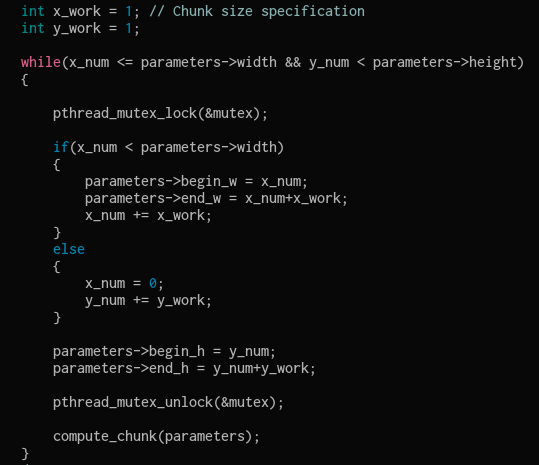
\includegraphics[width=.70\linewidth,scale=1]{./images/0.png} 
    \caption{Load-balanced implementation}
\end{figure}
\newpage
\thispagestyle{empty}

\section*{Performance results and comparison}
\subsection*{On our laptop(i5 2520M, 2Cores 4Threads)}

On the following figures, we cleary notice that the workload is unbalanced
with the \textit{naive} solution, for example the computation is actually
slower using 3 threads rather than 2.
On the other hand, with our balanced implementation the workload 
scale with the number of threads.

Note that with this 2C/4T machine we observe slower performances while 
using 5 or 6 threads, which is normal since the computation is using more 
threads that the machine actually has.

\begin{figure}[h]
    \centering
    \begin{tabular}{cc}
 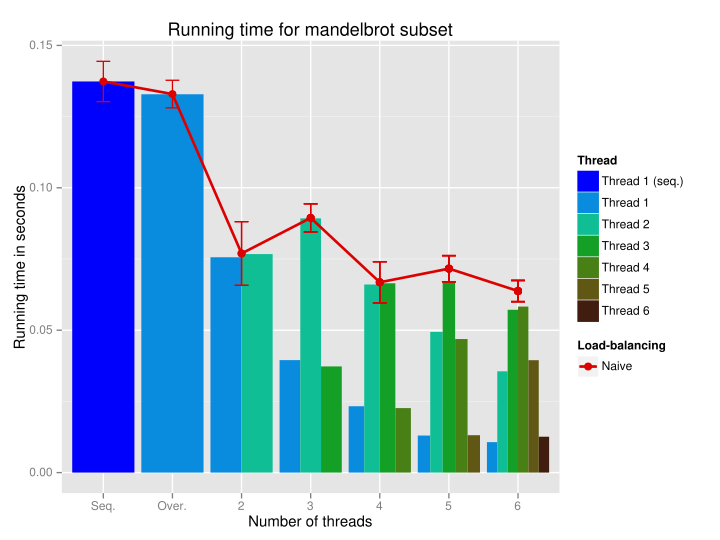
\includegraphics[width=.50\linewidth,scale=1]{./images/2.png} &
 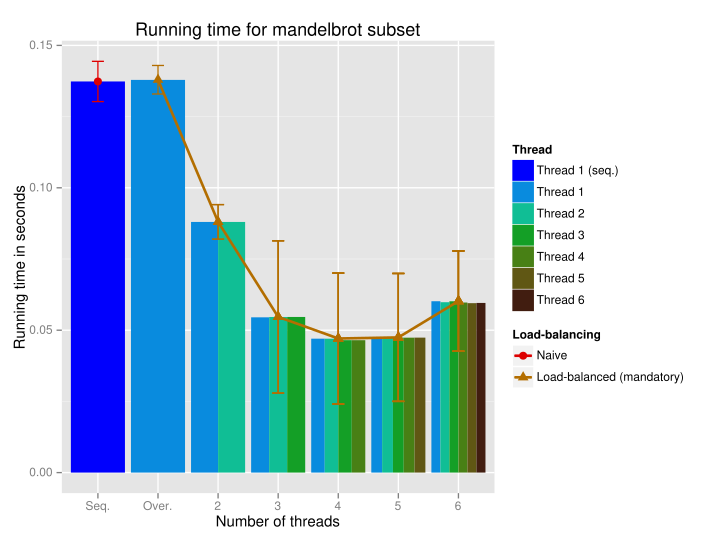
\includegraphics[width=.50\linewidth, scale=1.5]{./images/3.png} \\
      (a) & (b)
    \end{tabular}
    \caption{Naive (a) and Load-balanced (b)}
\end{figure}

\subsection*{On a multicore lab computer}


\begin{figure}[h]
    \centering
    \begin{tabular}{cc}
 %\includegraphics[width=.49\linewidth,scale=1]{./images/tab3.png} &
 %\includegraphics[width=.49\linewidth, scale=1.5]{./images/tab4.png} \\
      (a) & (b)
    \end{tabular}
    \caption{Naive (a) and Load-balanced (b)}
\end{figure}









  \cleardoublepage
  %\include{partie2}
  %\cleardoublepage
  %\include{partie3}
  %\cleardoublepage
  %\include{concl}
  %\cleardoublepage
\end{document}
